\documentclass{llncs}


%\usepackage[scaled=0.85]{beramono}
%\usepackage{libertine}
\usepackage[utf8]{inputenc}            % Enable UTF-8 encoding
\usepackage[T1]{fontenc}               % 8-bit output encoding
\usepackage{amsmath,amssymb,mathtools} % Maths typesetting
\usepackage{thmtools,thm-restate}      % restatable theorems, lemmas, etc...
\usepackage{mathpartir}                % Inference rules
\usepackage{mathwidth}                 % Render character sequences nicely in math mode
\usepackage{stmaryrd}                  % semantic brackets
\usepackage{xspace}                    % proper spacing for macros in text
\usepackage[hidelinks,pdftex]{hyperref}% Interactive PDF
\usepackage{listings}                  % Source code listings
\usepackage{url}
\usepackage[usenames,dvipsnames,svgnames,table]{xcolor}
\usepackage{subcaption}
\usepackage[misc]{ifsym}

\usepackage[numbers]{natbib}
\bibliographystyle{splncsnat}
%\setcitestyle{authoryear,square,semicolon}

%\input{multicore-ocaml.lststyle.tex}   % load Multicore OCaml listing style
%\lstset{style=multicore-ocaml}         % use Multicore OCaml style by default

\lstdefinestyle{sOcaml}{language=[Objective]Caml,
  literate={+}{{$+\:$}}1 {/}{{$/$}}1 % { * }{{$*$}}1
           {=}{{$=\ $}}1
           {>}{{$>$}}1 {<}{{$<$}}1
           {<>}{$\not=\ $}1
           {->}{{$\rightarrow$} }2 {>=}{{$\geq$}}2 {<-}{{$\leftarrow$}}2
           {<=}{{$\leq$}}2
           {=>}{{$\Rightarrow$}}2
           {+->}{{$\hookrightarrow$}}2
           {==>}{{$\mapsto$}}2
           {fn}{$\lambda$}1
           {|}{{$\mid$}}1
           {'a}{$\alpha$ }1
           {+'a}{$\textrm{+}\alpha$}1
           {'b}{$\beta$}1
           {+'b}{$\textrm{+}\beta$}1
           {'c}{$\gamma$}1
           {'e}{$\epsilon$}1
           {'w}{$\omega$}1
           {'w.}{$\forall\omega.\ $}2
           {t1}{t$_1$}2
           {t2}{t$_2$}2
           {vO}{v$_o$}1
           {vV}{v$_v$}1
           {\ .\ }{$\;\circ\;$}1
           {TRB}{\mbox{\ensuremath\lceil}}1
           {TRE}{\mbox{\ensuremath\rceil}}1
           {...}{\ldots}2
           %% {\#\#+}{\color{dred}}1
           %% {\#\#*}{\color{dgreen}}1
           %% {\#\#-}{\color{black}}1
           {\#\#\#}{{$\leadsto$}}3
}

\definecolor{weborange}{RGB}{255,165,0}
\definecolor{frenchplum}{RGB}{129,20,83}
\definecolor{eminence}{RGB}{108,48,130}
\definecolor{commentgreen}{RGB}{2,112,10}
\definecolor{mauve}{rgb}{0.88,0.69,1.0}

\lstset{
	style=sOCaml,
  basicstyle=\footnotesize\ttfamily,
  commentstyle=\color{OliveGreen},
  escapeinside={(**}{)},
  keywordstyle=\color{blue},
  language=[Objective]Caml,
	emph={Async,Await,Yield,Done,Error,Waiting,Accept,Recv,Send,Delayed,Completed,Break,Signal_handle,Some,None,TimerTick},
	emphstyle={\color{BurntOrange}},
  morekeywords={effect,continue,discontinue,perform,finally},
  stringstyle=\color{mauve},
  showstringspaces=false,
  breaklines=true,                    % allows line breaks
  tabsize=2,
}

\newcommand\blfootnote[1]{%
	\begingroup
	\renewcommand\thefootnote{}\footnote{#1}%
	\addtocounter{footnote}{-1}%
	\endgroup
}


% TODOs
\newcommand{\todo}[1]{{\par\noindent\small\color{red} \framebox{\parbox{\dimexpr\linewidth-2\fboxsep-2\fboxrule}{\textbf{TODO:} #1}}}}
\newcommand{\sam}[1]{{\par\noindent\small\color{red} \framebox{\parbox{\dimexpr\linewidth-2\fboxsep-2\fboxrule}{\textbf{Sam:} #1}}}}
\newcommand{\kc}[1]{{\par\noindent\small\color{red} \framebox{\parbox{\dimexpr\linewidth-2\fboxsep-2\fboxrule}{\textbf{KC:} #1}}}}
\newcommand{\dhil}[1]{{\par\noindent\small\color{red} \framebox{\parbox{\dimexpr\linewidth-2\fboxsep-2\fboxrule}{\textbf{Daniel:} #1}}}}


\lstMakeShortInline[columns=fullflexible]|

\begin{document}

\title{Concurrent System Programming with Effect Handlers}

\author{Stephen Dolan\inst{1} \and
				Spiros Eliopoulos\inst{3} \and
				Daniel Hillerström\inst{2} \and
				Anil Madhavapeddy\inst{1} \and
				KC Sivaramakrishnan\inst{1}(\Letter) \and
			  Leo White\inst{3}}

\institute{University of Cambridge
\and The University of Edinburgh
\and Jane Street Group}

\maketitle

\begin{abstract}
	Algebraic effects and their handlers have been steadily gaining attention as
	a programming language feature for composably expressing user-defined
	computational effects. While several prototype implementations of languages
	incorporating algebraic effects exist, Multicore OCaml incorporates effect
	handlers as the primary means of expressing concurrency in the language. In
	this paper, we make the observation that effect handlers can elegantly
	express particularly difficult programs that combine system programming and
	concurrency without compromising performance. Our experimental results on a
	highly concurrent and scalable web server demonstrate that effect handlers
	perform on par with highly optimised monadic concurrency libraries, while
	retaining the simplicity of direct-style code.
\end{abstract}

\section{Introduction}

\blfootnote{\Letter~\texttt{sk826@cl.cam.ac.uk}}

Algebraic effect handlers are a modular foundation for effectful programming,
which separate the \emph{operations} available to effectful programs from their
concrete implementations as \emph{handlers}. Effect handlers provide a modular
alternative to monads~\citep*{Moggi91,Wadler92} for structuring effectful
computations. They achieve the separation between operations and their handlers
through the use of delimited continuations, allowing them to pause, resume and
switch between different computations. They provide a structured interface for
programming with delimited continuations~\citep*{ForsterKLP17}, and can
implement common abstractions such as state, generators, async/await, promises,
non-determinism, exception handlers and backtracking search. Though originally
studied in a theoretical setting~\cite{PlotkinP01,PlotkinP13}, effect handlers
have gained practical interest with several prototype implementations in the
form of libraries, interpreters, compilers and runtime
representations~\citep*{BauerP15,Brady13,DolanWSYM15,HillerstromL16,KammarLO13,KiselyovI15,Leijen17,LindleyMM17}.

However, the application space of effect handlers remains largely unexplored. In
this paper we explore the applicability of effect handlers to concurrent system
programming in Multicore OCaml. While Multicore OCaml supports shared-memory
parallel programming, this paper restricts its focus to concurrency i.e.
overlapped execution of tasks, leaving parallelism outside our scope.

\section{Motivation}

Multicore OCaml~\citep*{DolanWM14} incorporates effect handlers as the primary
means of expressing concurrency in the language. The modular nature of effect
handlers allows the concurrent program to abstract over different scheduling
strategies~\citep*{DolanWSYM15}. Moreover, effect handlers allow concurrent
programs to be written in \emph{direct-style} retaining the simplicity of
sequential code as opposed to callback-oriented style (as used by e.g.
Lwt~\citep*{Vouillon08} and Async~\citep*{Minsky13}). In addition to being more
readable, direct-style code tends to be easier to debug; unlike
callback-oriented code, direct-style code uses the stack for function calls, and
hence, backtraces can be obtained for debugging. Indeed, experience from Google
suggests that as well as making the code more compact and easier to understand
(particularly important when thousands of developers touch the code),
direct-style code can perform as well or better than callback-oriented
code~\citep*{Barroso2017}.

Some of the benefits of direct-style code can be achieved by rewriting
direct-style functions into callbacks, using syntactic sugar
such as Haskell's \verb|do|-notation for monads or F\#'s
|async/await|~\citep*{syme2011fsharp}.  However, this separates functions which
use such rewriting from those that do not, leading to awkward mismatches and
code duplication: for instance, Haskell
provides |mapM|, |filterM| and |foldM| because the ordinary |map|, |filter| and
|foldl| functions do not work with monadic arguments. By contrast, effect
handlers do not introduce an incompatible type of function.

In Multicore OCaml, the user-level thread schedulers themselves are expressed
as OCaml libraries, thus minimising the secret sauce that gets baked into
high-performance multicore runtime systems~\citep*{KcHMP16}. This modular
design allows the scheduling policy to be changed by swapping out the
scheduler library for a different one with the same interface. As the
scheduler is a library, it can live outside the compiler distribution and
be tailored to application requirements.

However, the interaction between user-level threading systems and the operating
system services is difficult. For example, the Unix \texttt{write()} system call
may block if the underlying buffer is full. This would be fine in a
sequential program or a program with each user-level thread mapped to a unique
OS thread, but with many user-level threads multiplexed over a single OS thread, a
blocking system call blocks the entire program. How then can we
safely allow interaction between user-level threads and system services?

Concurrent Haskell~\citep*{MarlowPJT04}, which also has user-level
threads, solves the problem with the help of specialised runtime system
features such as safe FFI calls and bound threads. However, implementing
these features in the runtime system
warrants that the scheduler itself be part of the runtime system, which is
incompatible with our goal of writing thread schedulers in OCaml. Attempts to
lift the scheduler from the runtime system to a library in the high-level
language while retaining other features in the runtime system lead to further
complications~\citep*{KcHMP16}.

\noindent Our goals then are:

\begin{itemize}
	\item Retain the simplicity of direct-style code for concurrent OCaml
		programs.
	\item Allow user-level thread schedulers to be
		written in OCaml as libraries.
	\item Allow safe interaction between user-level threads and the operating system.
	\item Perform as well as or better than existing solutions.
\end{itemize}

We observe that algebraic effects and their handlers can meet all of
these goals. In particular, we introduce \emph{asynchronous effects}
and their handlers, and show how they elegantly solve the interaction
between user-level threads and operating system services. This paper
makes the following contributions:

\begin{itemize}
	\item We introduce effect handlers for Multicore OCaml and illustrate their
		utility by constructing a high-performance asynchronous I/O library that
		exposes a direct style API (Section~\ref{sec:effect_handlers}).
	\item We show how \emph{asynchronous effects} provide a clean interface to
		difficult-to-use operating system services, such as signal handling and
		asynchronous notification of I/O completion, and demonstrate how effect
		handlers enable scoped interrupt handling
		(Section~\ref{sec:async_effects}).
	\item We evaluate the performance of effect handlers in OCaml by implementing
		a highly scalable web server and show that Multicore OCaml effect handlers
		are efficient (Section~\ref{sec:results}).
\end{itemize}

After the technical content of the paper in
Sections~\ref{sec:effect_handlers}, \ref{sec:async_effects}, and
\ref{sec:results}, we discuss related work in
Section~\ref{sec:related_work} and our conclusions in
Section~\ref{sec:conclusions}.

\section{Algebraic effects and their handlers}
\label{sec:effect_handlers}

Since the primary motivation for adding effect handlers in Multicore
OCaml is concurrency, we introduce effect handlers in constructing an
asynchronous I/O library which retains the simplicity of direct-style
programming~\footnote{A comprehensive list of example programs written
  using effect handlers in Multicore OCaml is available at
  \url{https://github.com/kayceesrk/effects-examples}}.

\subsection{Concurrency}

We start with an abstraction for creating asynchronous tasks and waiting
on their results. We use the term \emph{fiber} to indicate a lightweight
user-level thread to distinguish it from kernel threads.
\begin{lstlisting}
val async : ('a -> 'b) -> 'a -> 'b promise
(* [async f v] spawns a fiber to run [f v] asynchronously. *)

val await : 'a promise -> 'a
(* Block until the result of a promise is available. Raises exception [e] if the promise raises [e]. *)

val yield : unit -> unit
(* Yield control to other fibers. *)
\end{lstlisting}

Multicore OCaml extends OCaml with the ability to declare user-defined effects
with the help of the |effect| keyword. Since |async|, |await| and |yield| are
effectful operations, we declare them as follows:

\begin{lstlisting}
effect Async : ('a -> 'b) * 'a -> 'b promise
effect Await : 'a promise -> 'a
effect Yield : unit
\end{lstlisting}

The first declaration says that |Async| is an effect which is parameterised by
a pair of a thunk and a value, and returns a promise as a result when
performed. |Await| is parameterised by a promise and returns the result.
|Yield| is a nullary effect that returns a unit value. To be precise, these
declarations are \emph{operations} of a single built-in effect type |'a eff| in
Multicore OCaml. Indeed, these declarations are syntactic sugar for
extending the built-in extensible variant type |'a eff|:

\begin{lstlisting}
type _ eff +=
  | Async : ('a -> 'b) * 'a -> 'b promise eff
  | Await : 'a promise -> 'a eff
  | Yield : unit eff
\end{lstlisting}

Effects are performed with the |perform : 'a eff -> 'a| primitive, which
performs the effect and returns the result. We can now define the functions
|async|, |await| and |yield| as:

\begin{lstlisting}
let async f v = perform (Async (f,v))
let await p   = perform (Await p)
let yield ()  = perform Yield
\end{lstlisting}


\begin{figure}
\begin{lstlisting}[numbers=left,numbersep=5pt,numberstyle=\sffamily\tiny]
type 'a _promise = Done of 'a | Error of exn
                 | Waiting of ('a, unit) continuation list

type 'a promise = 'a _promise ref

let run main v =
  let run_q = Queue.create () in
  let enqueue f = Queue.push f run_q in
  let run_next () =
    if Queue.is_empty run_q then ()
    else Queue.pop run_q ()
  in
  let rec fork : 'a 'b. 'a promise -> ('b -> 'a) -> 'b -> unit =
    fun p f v ->
      match f v with
      | v ->
          let Waiting l = !p in
          List.iter (fun k ->
            enqueue (fun () -> continue k v)) l;
          p := Done v;
          run_next ()
      | exception e ->
          let Waiting l = !p in
          List.iter (fun k ->
            enqueue (fun () -> discontinue k e)) l;
          p := Error e;
          run_next ()
      | effect (Async (f,v)) k ->
          let p = ref (Waiting []) in
          enqueue (fun () -> continue k p);
          fork p f v
      | effect (Await p) k ->
          match !p with
          | Done v -> continue k v
          | Error e -> discontinue k e
          | Waiting l -> p := Waiting (k::l); run_next ()
      | effect Yield k ->
          enqueue (fun () -> continue k ());
          run_next ()
  in
  fork (ref (Waiting [])) main v
\end{lstlisting}
\caption{A simple scheduler, implemented with effects}
\label{fig:scheduler}
\end{figure}

These effects are interpreted by an effect handler, as shown in
Figure~\ref{fig:scheduler}. A promise (lines 1--6) is either completed
successfully |Done v|, failed with an exception |Error e| or still pending
|Waiting l|, with a list of fibers waiting on it for completion. The function
|run| (line 8) is the top-level function that runs the |main| concurrent
program. |run_q| is the queue of concurrent fibers ready to run. The effect
handler itself is defined in the lines 17--38. An effect handler comprises of
five clauses -- a value clause, an exception clause, and three clauses that
handle the effects |Async|, |Await| and |Yield|.

Effect clauses are of the form |effect e k| where |e| is the effect and |k| is
the continuation of the corresponding |perform| delimited by this handler. |k|
is of type |('a, 'b)|~|continuation|, representing a continuation waiting for
a value of type |'a| and returning a value of type |'b| when resumed. There are
two primitives operating on continuations: |continue k x| resumes the
continuation |k| where it left off, returning the value |x| from |perform|,
while |discontinue k exn| resumes the continuation |k| by raising the exception
|exn| from |perform|.

In the case of an |Async (f,v)| effect (lines 28--31), we create a new promise
value |p| which is initially waiting to be completed. We set up the original
fibers, represented by continuation |k|, to resume with the promise using the
|continue| primitive. Finally, we recursively call |fork| to run the new fiber
|f v|. Since Multicore OCaml uses so-called \emph{deep handlers}, the
continuation |k| references its surrounding handler, and so we need not write
another |match| expression when |continue|-ing |k| (See Kammar et
al.~\citep*{KammarLO13} for more on deep vs. shallow handlers).

In the case of |Await p|, we check whether the promise is complete. If
successful, we immediately resume with the value, and if failed, we use the
|discontinue| primitive to resume the continuation by raising an exception.
Otherwise, we block the current fiber on
the promise and resume the next fiber from the scheduler. In the case of
|Yield| effect, we enqueue the current fiber and run the next available fiber.
In the case of a fiber successfully running to completion (lines 18--23) or
raising an exception (lines 24--29), we update the promise, wake up the waiting
fibers and resume the next available fiber.

\subsection{Implementing effect handlers}

Unlike other languages that incorporate effect handlers, effects in Multicore
OCaml are unchecked. That is, there is no static check for whether all the
possible effects have been handled in the program. As a result, a fiber that
performs an unhandled effect is discontinued with |Unhandled| exception.

There are several alternatives to implement the continuations in effect
handlers including free monadic
interpretations~\citep*{KiselyovI15,KiselyovSS13,WuSH14}, CPS
translations~\citep*{HillerstromLAS17,Leijen17}, and runtime strategies.
Multicore OCaml chooses the latter and uses a custom stack
layout, efficiently supported by the runtime system.
We observe that many effect handlers do not resume the
continuations more than once, and support only linear continuations by
default, which can be implemented efficiently~\citep*{DolanWSYM15}. We also
support explicit copying for non-linear use of continuations.

\subsection{Adding I/O}
\label{sec:effect-io}

Next let us add support for the following I/O operations:

\begin{lstlisting}
val accept : file_descr -> file_descr * sockaddr
val recv : file_descr -> bytes -> int -> int
        -> msg_flag list -> int
val send : file_descr -> bytes -> int -> int
        -> msg_flag list -> int
\end{lstlisting}

These functions have the \emph{same} signature as their counterparts in the
|Unix| module. However, invoking any of these functions may block the kernel
thread until the I/O operation is complete. In a user-level threaded system this
would block the scheduler, preventing other fibers from running.

The standard solution to this problem is to use an event loop, suspending each
task performing a blocking I/O operation, and then multiplexing the outstanding I/O
operations through an OS-provided blocking mechanism such as |select|, |epoll|,
|kqueue|, |IOCP|, etc. Such asynchronous, non-blocking code typically warrants
callback-oriented programming, making the continuations of I/O operations
explicit through explicit callbacks (à la JavaScript) or concurrency monad (Lwt
and Async libraries for OCaml). The resultant code is arguably messier and
more difficult to understand than direct-style code.

Effect handlers lets us retain direct-style while still allowing the use of
event loops. Below, we shall just consider |accept|. The
other functions are similar. As earlier, we start by declaring an effect for an
|accept| function: |effect Accept : file_descr -> (file_descr * sockaddr)|. The
handler for |Accept| is:

\begin{lstlisting}
| effect (Accept fd) k ->
    (match Unix.accept fd with
     | (newfd, sockaddr) ->
        continue k (newfd, sockaddr)
     | exception Unix_error(EWOULDBLOCK, _, _) ->
        record_waiting fd k; run_next ())
\end{lstlisting}

If there is a waiting connection, |Unix.accept| returns it and we
resume the continuation. If not, |Unix.accept| raises the
|EWOULDBLOCK| error, and we record that the fiber is waiting to accept
and switch to the next thread from the scheduler queue. The
|send| and |recv| operations have similar handler implementations.

\begin{lstlisting}
let run_next () =
  if Queue.is_empty run_q then
		if io_is_pending () then begin
			wait_until_io_ready (); do_io (); run_next ()
		end else () (* done *)
	else Queue.pop run_q ()
\end{lstlisting}

Correspondingly, the |run_next| function is updated such that it first runs all
the available threads, and then if any I/O is pending it waits until at least
one of the I/O operations is ready, and then tries to perform the I/O and
continue. If the scheduler queue is empty, and there is no pending I/O, then
the scheduler returns. The library blocks on I/O only if there are no ready
threads and there are pending I/O operations.

Using this API, we can write a simple server that echoes client messages:

\begin{lstlisting}
let rec echo_server sock =
	let sent = ref 0 in
  let msg_len = (* receive message *)
    try recv sock buffer 0 buf_size [] with
    | _ -> 0 (* Treat exceptions as 0 length message *) in
  if msg_len > 0 then begin
    (* echo message *)
    (try while !sent < msg_len do
      let write_count =
        send sock buffer !sent (msg_len - !sent) [] in
      sent := write_count + !sent
    done with _ -> ()); (* ignore send failures *)
    echo_server sock
  end else close sock (* client left, close connection *)
\end{lstlisting}

The details of the code are not important, but observe that the code is in
direct-style and moreover is the \emph{same} code for the synchronous, blocking
echo server. Furthermore, since the following code is asynchronous, the two
echo servers on |sock1| and |sock2| do not block each other:

\begin{lstlisting}
run (fun () ->
      async echo_server sock1; async echo_server sock2) ()
\end{lstlisting}

\subsection{Default handlers}
\label{sec:default-handlers}

For an invocation of an effectful operation to be meaningful it must happen in
the scope of an appropriate handler. A default handler is a convenient
mechanism for ensuring that an operation invocation is always meaningful even
when not in scope of a handler. A default handler provides a \emph{default}
interpretation of an operation. This interpretation is chosen if no other
appropriate handler encloses the invocation context. In other words, a default
handler can operationally be understood as a top level handler which encloses
the entire program context including itself.
%
As a concrete example we can give a default synchronous semantics for
|Accept|
%
\begin{lstlisting}
effect Accept : file_descr -> (file_descr * sockaddr)
  with function Accept fd -> Unix.accept fd
\end{lstlisting}
%
In Multicore OCaml a default handler is declared along with the
effectful operation it is handling using the familiar |function|
construct. In contrast to a regular effect handler, a default handler
does not expose the continuation of the operation to the programmer,
rather, the continuation is implicitly applied to the body
clause(s). This particular design admits an efficient implementation,
since every continuation invocation in a default handler is guaranteed
to be in tail position. Thus the runtime does not need to allocate a
continuation, it can simply return the value produced by the default
handler clause. As a consequence an invocation of a default handler
amounts to a function call. This makes it possible for effectful
libraries to remain \emph{performance backwards compatible} with
programs that do not use regular effect handlers.
% %
% Thus providing a convenient abstraction for exposing effectful
% functions in a type system without effect tracking.

% The observation that the echo server is the same as the one for synchronous,
% blocking code is an important one. In particular, we can recover synchronous
% behavior with the help of default handlers. Multicore OCaml allows effect
% declarations to express default behavior for unhandled effects -- effects which
% do not have an enclosing handler. We can define the default behavior of
% |Await|, |Async|, |Yield| and |Accept| as its synchronous counterpart:

Continuing, we can also obtain the synchronous counterparts to
|Await|, |Async|, and |Yield| by giving them all a default synchronous
semantics, i.e.
\begin{lstlisting}
effect Async : ('a -> 'b) * 'a -> 'b promise
  with function Async (f, v) ->
	  match f v with
		| v -> ref (Done v)
		| exception e -> ref (Error e)

effect Await : 'a promise -> 'a
  with function Await (ref (Done v)) -> v
              | Await (ref (Error e)) -> raise e

effect Yield : unit with function Yield -> ()
\end{lstlisting}

If a default handler raises an exception, then the fiber is discontinued with
that exception. Furthermore, if a default handler performs an effect then the
default handler of that effect is invoked.
% If the default handler returns a value (raises an exception), then the fiber
% continues (dis-continues) with the value (exception). If the default handler
% performs an effect, then the default handler of that effect is invoked. We can
% implement the default handler for |Send| and |Recv| effect in a similar
% fashion. With default handlers, the program
If we define the default implementations of |Send| and |Recv| in a
similar way then by using default handlers the following program
behaves exactly like its synchronous counterpart.
\begin{lstlisting}
async echo_server sock1; async echo_server sock2
\end{lstlisting}

\section{Programming with resources and effects}
\label{sec:async_effects}

Systems programming generally involves the manipulation of scarce
resources such as file handles, connections and locks. Such resources
are inherently linear, stateful values: once a file handle is closed,
it cannot be used again.

Ordinary straight-line imperative code is not enough to use resources
correctly in the presence of exceptions, let alone effects.
For instance, the following code leaks an unclosed file handle if
|do_stuff_with f| raises an exception:
\begin{lstlisting}
let f = open_in "data.csv" in
do_stuff_with f;
close_in f
\end{lstlisting}
We need to ensure that the file handle is closed, even if an
exception is raised:
\begin{lstlisting}
let f = open_in "data.csv" in
match do_stuff_with f with
| () -> close_in f
| exception e -> close_in f; raise e
\end{lstlisting}
Note that the initial |open_in| occurs outside the exception handler -
if opening the file fails with an exception, we need not close
it. This idiom or something equivalent is widespread, often with
syntactic support as |try-finally|.

However, note an implicit assumption in this code, that if |do_stuff_with f|
terminates then it does so only once. If the computation |do_stuff_with f| were
to return twice (by allowing a continuation captured inside |f| to be
resumed twice), then the cleanup code (|close_in f| in this example) would
incorrectly run multiple times. If the computation |do_stuff_with_f| were to
continue execution after the cleanup code had run, its operations would have
unexpected effects.

As well as the performance advantages mentioned above, this is
the other major reason that our continuations are linear. By
preserving the linearity of computations (operations that are begun
once do not complete twice), we allow resource-manipulating code to
work correctly in the presence of effects.

Some interesting examples of programming with effects and handlers
(such as backtracking) are incompatible with this approach, since they
rely on continuations to be usable more than once. To support
experimenting with such examples, we do provide a primitive to allow
re-use of continuations, with the proviso that it is not safe in
general when used with code that handles resources.

The linearity of computations is implicit in OCaml without effect
handlers, but once continuations appear as first-class values the
possibility of using them twice arises. OCaml does not have the linear
types necessary to prevent this statically (and we are not proposing
to add them), so we must enforce linearity dynamically. Ensuring that
a continuation is not used twice is easy enough, by keeping a bit of
state in the continuation, updated by |continue| and
|discontinue| so that subsequent resumptions fail. Ensuring that
a continuation is not simply discarded is harder: the system must
detect when a continuation is being garbage-collected, and
|discontinue| it with a special exception so that resource
cleanup code runs.

\subsection{Asynchronous exceptions}

Correct use of resources is much more difficult in the presence of
\emph{asynchronous exceptions}. For example, on Unix-like systems when
the user of a command-line program presses |Ctrl-C| the
|SIGINT| signal is sent. By default, this
terminates the program. However, programs may indicate that they can
handle this signal, for instance by cancelling a long-running
task and accepting user input again.

In OCaml, programs indicate willingness to handle |SIGINT| by
calling |Sys.catch_break true|. From that point onwards, the
special exception |Sys.Break| may be raised at essentially any
point in the program, if the user presses |Ctrl-C|.
Unfortunately, the try-finally idiom does not clean up correctly in
this case:
\begin{lstlisting}
let f = open_in "data.csv" in
match do_stuff_with f with
| () -> close_in f
| exception e -> close_in f; raise e
\end{lstlisting}
If |Sys.Break| is raised just after |open_in| returns but before the
|match| statement is entered, then the file handle will never be
closed. To eliminate this possibility, we need to temporarily disable
asynchronous exceptions. Suppose we introduce two functions |set_mask|
and |clear_mask|, to disable (\emph{mask}) and re-enable asynchronous
exceptions. Our second attempt at resource handling looks like:
\begin{lstlisting}
set_mask ();
let f = open_in "data.csv" in
match clear_mask (); do_stuff_with f; set_mask () with
| () -> close_in f; clear_mask ()
| exception e -> set_mask (); close_in f; clear_mask (); raise e
\end{lstlisting}
Correctly placing calls to |set_mask| and |clear_mask| is a
very tricky business. Indeed, the above code has a serious bug: if
|open_in| fails with an ordinary synchronous exception (because
e.g. the file is not found), then asynchronous exceptions will never
be unmasked.

Instead, we follow the good advice of Marlow et al. in the design of
Haskell's asynchronous exceptions~\citep*{Marlow2001async},
and prefer instead \emph{scoped combinators}:
\begin{lstlisting}
mask (fun () ->
  let f = open_in "data.csv" in
  match unmask (fun () -> do_stuff_with f) with
  | () -> close_in f
  | exception e -> close_in f; raise e)
\end{lstlisting}
The changes to the masking state made by |mask| and |unmask|
apply only to one scope, and are automatically undone, making it
impossible to accidentally leave asynchronous exceptions masked.
The presence of |unmask| allows a further improvement to the
semantics: we model the asynchronous exception |Sys.Break| as being
raised not by whatever code happened to be executing when |Ctrl-C| was
pressed, but by the nearest enclosing |unmask|. This ensures that exception
handlers for asynchronous exceptions need not be treated specially. In
particular, the follow code cannot fail, no matter when |Ctrl-C| is
pressed:
\begin{lstlisting}
match 1 + 1 with
| n -> n
| exception Sys.Break -> failwith "what?"
\end{lstlisting}

% mention the subtlety about nested mask?

\subsection{Signal handling and asynchronous effects}
\label{sec:signals}

Even with the scoped masking combinators, it is difficult and
unpleasant to write code that correctly manipulates resources in the
presence of asynchronous exceptions. For this reason, many systems
choose instead to poll for cancellation requests, instead of being
interrupted with one. That is, instead of a |Sys.Break| exception
being raised, the programmer manually and regularly checks a mutable
boolean |cancellation_flag|, which is asynchronously set to |true|
when the user presses |Ctrl-C| (This check may be combined with other
system facilities: one common choice is that cancellation is checked
at all I/O operations, since the program must handle failures there
anyway).

On Unix-like systems, it is possible to implement this behaviour using
a \emph{signal handler}, which is a callback invoked when a signal is
raised (e.g. by the user pressing |Ctrl-C|). In OCaml, these can
be installed using the function |Sys.set_signal|. In fact, the
behaviour of the previously-mentioned |Sys.catch_break| is
implemented by installing a signal handler that raises |Sys.Break|:
\begin{lstlisting}
set_signal sigint (Signal_handle(fun _ -> raise Break))
\end{lstlisting}
Synchronous cancellation can be implemented using a signal handler
that sets a cancellation flag:
\begin{lstlisting}
let cancellation_flag = ref false
let is_cancelled () = !cancellation_flag
let () =
  set_signal sigint (Signal_handle(fun _ ->
    cancellation_flag := true))
\end{lstlisting}

By removing the possibly of cancellation except at designated points,
the imperative parts of the system become safer and easier to write. However, as
Marlow et al.~\citep*{Marlow2001async} note, for the purely functional parts of the
system asynchronous cancellation is both necessary and just as safe as synchronous:
necessary, because inspecting the mutable cancellation state breaks
referential transparency, and safe, because purely functional code
holds no resources and pure computations can be abandoned without issue.

In order to call a pure function from imperative code while
maintaining prompt cancellation, we need to switch from synchronous
(polling) cancellation to asynchronous cancellation and back, by
providing a combinator:
\begin{lstlisting}
async_cancellable : (unit -> 'a) -> (unit -> 'a option)
\end{lstlisting}
Normally, |async_cancellable f| returns |Some (f ())|. However, the
computation |f| may be cancelled asynchronously, causing
|async_cancellable f| to return |None|, ensuring that asynchronous
cancellation does not affect the caller.

Our first attempt at such a mechanism looks like:
\begin{lstlisting}
let sync_handler = Signal_handle (fun _ ->
  cancellation_flag := true)
let async_handler = Signal_handle (fun _ ->
  raise Break)
let async_cancellable f =
  mask (fun () ->
    match
      set_signal sigint async_handler;
      let result = unmask f in
      set_signal sigint sync_handler;
      result
    with
    | x -> Some x
    | exception Break -> None)
\end{lstlisting}
This code is tricky, due to its delicate
mutation of global state. It is very similar to the code we saw
earlier using |set_mask| and |clear_mask|, and even has the
same bug: it leaves the wrong signal handler in place if
|f| raises an exception.

As before, scoped combinators make such code easier to get right (or,
more accurately, harder to get wrong). To this end, we introduce
\emph{asynchronous effects}, which are effects that can be performed
asynchronously, just as asynchronous exceptions can be raised
asynchronously. By treating |Break| as an asynchronous effect, we
can mix synchronous and asynchronous cancellation reliably.

For synchronous cancellation, we handle
the |Break| effect by setting a flag:
\begin{lstlisting}
let cancellation_flag = ref false
let sync_cancellable f =
  mask (fun () ->
    match unmask f with
    | result -> result
    | effect Break k ->
      	cancellation_flag := true; continue k ())
\end{lstlisting}
Asynchronously-cancellable code can be implemented by handling the
|Break| effect and discarding the continuation. Since effect handlers
delimit the continuation, the asynchrony is limited to the specified
function.
\begin{lstlisting}
let async_cancellable f =
  mask (fun () ->
    match unmask f with
    | result -> Some result
    | effect Break k -> None)
\end{lstlisting}
Instead of having a single global callback as the current signal
handler, asynchronous effects allow handlers to delimit their scope
and nest correctly.

\subsection{Managing multiple computations with asynchronous effects}

Unlike signal handlers, asynchronous effects get an explicit
representation of the computation they interrupted by way of the
continuation |k|. While signal handlers can only resume the
computation or abandon it (by raising an exception), effect handlers
have other options available. For instance, a scheduler which
maintains a collection of tasks can switch to another task when handling
an asynchronous effect, just as the scheduler in Fig.~\ref{fig:scheduler}
does for the synchronous |Yield| effect. Using
asynchronous effects the cooperative scheduler of Fig.~\ref{fig:scheduler} can be
made preemptive, by asking the operating system to provide a periodic
timer signal (using e.g. the Unix |timer_create| API), and adding a
new clause to the scheduler:
\begin{lstlisting}
| effect TimerTick k -> enqueue (continue k); run_next()
\end{lstlisting}

\subsection{Asynchronous I/O notifications}

Operating systems provide several different I/O interfaces.  The
simplest is the direct-style \emph{blocking I/O}, in which the program
calls operating-system functions which do not return until the
operation completes. This allows a straightforward style of
programming in which the sequence of I/O operations matches the flow
of the code. We aim to support this style of programming using
alternative operating system interfaces that allow multiple I/O
operations to be overlapped.

In Section~\ref{sec:effect-io}, we saw one way of accomplishing this
with effects, by using multiplexing mechanisms like
|select|, |poll|, etc., which block until one of several file
descriptors is ready. An alternative is
\emph{asynchronous I/O}, in which multiple operations are submitted to
the operating system, which overlaps their execution. However,
applications written using asynchronous I/O tend to have complex
control flow which does not clearly explain the logic being
implemented, due to the complexity of handling the operating system's
asynchronous notifications of I/O completion.

We propose effects and handlers as a means of writing direct-style I/O
code, but using the asynchronous operating system interfaces. We
introduce two new effect operations: |Delayed|, which describes an
operation that has begun and will complete later, and |Completed|,
which describes its eventual completion. Both of these take an integer
parameter, which identifies the
particular operation.

Potentially long-running operations like |read| perform the |Delayed|
effect, indicating that the operation has been submitted to the
operating system but has not yet completed. Later, upon receipt of an
operating-system completion notification, the asynchronous effect
|Completed| is performed.

Using this mechanism, support for asynchronous completions can be
added to the scheduler of Fig.~\ref{fig:scheduler} by adding clauses
for the |Delayed| and |Completed| effects, where |ongoing_io| is an
initially empty hash table:
\begin{lstlisting}
| effect (Delayed id) k ->
  Hashtbl.add ongoing_io id k
| effect (Completed id) k ->
  let k' = Hashtbl.find ongoing_io id in
  Hashtbl.remove ongoing_io id;
  enqueue (fun () -> continue k ());
  continue k' ()
\end{lstlisting}
In this sample, the continuation |k| of the |Delayed| effect is the
continuation of the code performing the I/O operation, which instead
of being immediately invoked is stored in a hash table until it can be
invoked without blocking.

The continuation |k| of the |Completed| effect is the continuation of
whichever fiber was running when the I/O completed. This scheduler
chooses to preempt that fiber in favour of the fiber that performed the
I/O. Equally, the scheduler could give
priority to the running fiber, by swapping |k| and |k'|
in the last lines.

\section{Results}
\label{sec:results}

So far we have presented what we believe are compelling applications of effect
handlers for elegant system programming. However, none of that would matter if
the resultant programs were unacceptably slower compared to extant solutions.
Hence, in this section, we evaluate the performance of a web server built with
effect handlers against existing production-quality web servers.

We have implemented an effect-based asynchronous I/O library,
|aeio|~\citep*{aeio}, that exposes a direct-style API to the clients. At its
core, |aeio| uses the main loop engine from the Lwt library using the
libev\footnote{\url{http://software.schmorp.de/pkg/libev.html}} event loop
(using {\em epoll} in our experiments). For the OCaml web server, we use
|httpaf|, which is a high performance, memory efficient, and scalable web
server that uses the Async library~\citep*{Minsky13} (also using {\em epoll} as
its I/O system call). We then extended |httpaf| and implemented an effect
handler based backend using |aeio|. The configurations we use for the
evaluation are:

\begin{itemize}
	\item {\bf Effect:} Effect-based version which uses |httpaf| with |aeio| on
		the Multicore OCaml compiler. The Multicore OCaml compiler was
		forked off vanilla OCaml version 4.02.2.
	\item {\bf Async:} Vanilla OCaml version 4.03.0, using |httpaf| + Async 113.33.03.
	\item {\bf Go:} Go 1.6.3 version of the benchmark using |net/http| package.
\end{itemize}
For comparison, all three configurations were constrained to only one
core (using the |GOMAXPROCS| variable in the case of Go).

The evaluations were done on a 3 GHz Intel Core i7 with 16 GB of main memory
running 64-bit Ubuntu 16.10. The client workload was generated by the
|wrk2|\footnote{\url{https://github.com/giltene/wrk2}} program. Each |wrk2| run
uses a fixed number of client connections that issues requests at a
constant rate, and measures request latency and throughput.

\begin{figure}
	\centering
	\begin{subfigure}[t]{0.48\textwidth}
		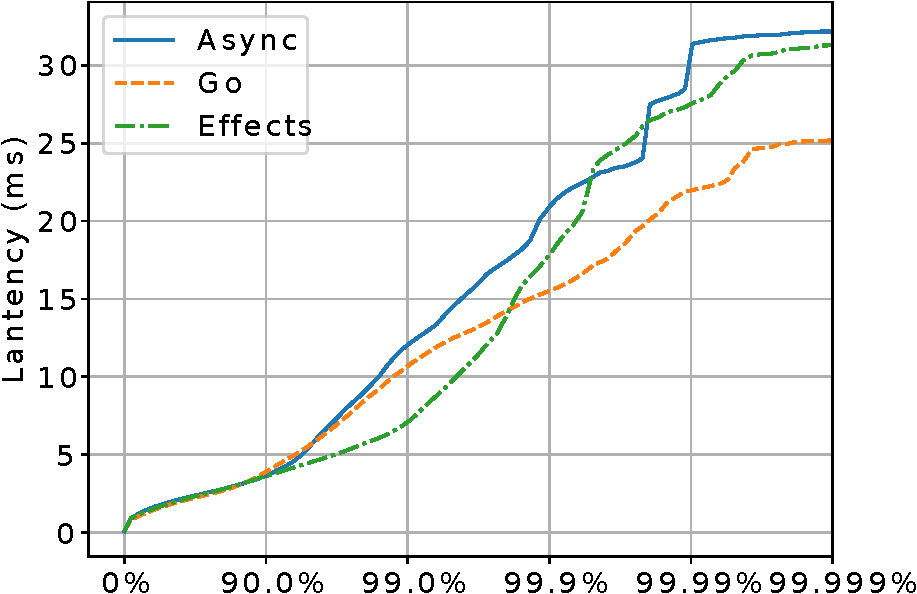
\includegraphics[width=0.99\textwidth]{graphs/latency_c1k_r10k.pdf}
		\caption{Medium contention: 1k connections, 10k requests/sec}
		\label{grf:c1k_r10k}
	\end{subfigure}
	\begin{subfigure}[t]{0.48\textwidth}
		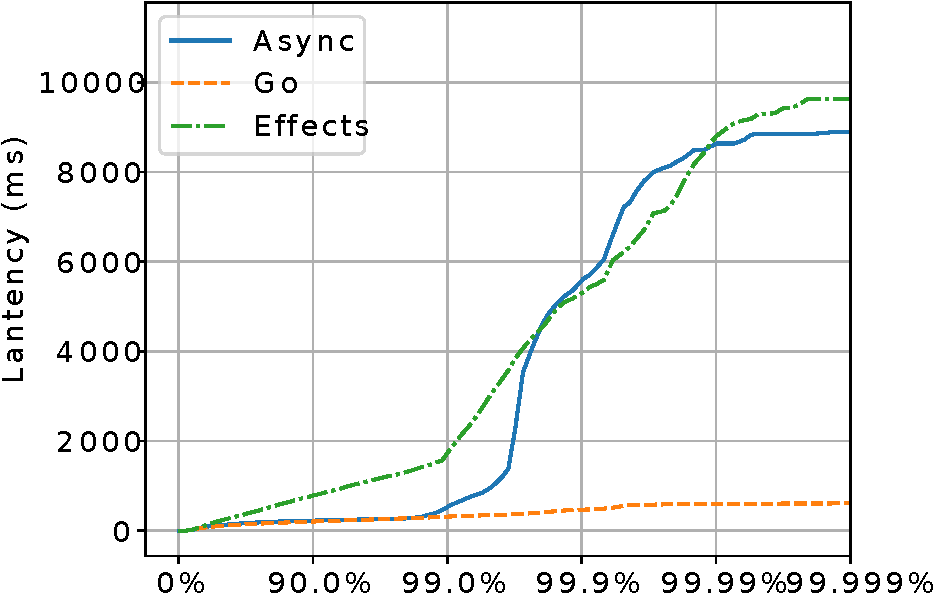
\includegraphics[width=\textwidth]{graphs/latency_c10k_r30k.pdf}
		\caption{High contention: 10k connections, 30k requests/sec}
		\label{grf:c10k_r30k}
	\end{subfigure}
	\caption{Latency profile of client requests}
	\label{grf:latency}
\end{figure}

Figure~\ref{grf:latency} shows the latency profiles for 1 minute runs under two
different configurations. At 1k connections and 10k requests per second, the
effect implementation performs marginally better than Async. Go performs the
best with all requests satisfied within 27 ms. The average request latency of
effect configuration is 2.127 ms over 587969 requests. Under this
configuration, the observed throughput is between 9780 and 9800 requests per
second in all of the configurations.

At high loads, the performance degrades substantially in every
configuration, but it is worse in the OCaml implementations. The
average latency for satisfying a client request increases to 333.40 ms
in the effect case, while it is 139 ms in async and 107.25 ms in
Go. While Go achieved 17389 requests per second, Async and effect
implementations achieved only 16761 and 15440 requests per second,
respectively. This indicates that there is room for
optimisations. Multicore OCaml has a new garbage collector, which has
not been tuned to the extent of vanilla OCaml and Go. We strongly
suspect that garbage collector optimisation and tuning would lead to
performance improvements. Importantly, the tail latencies of both OCaml implementations (the
vanilla Async and our effect-based server) were comparable in both
configurations, indicating that there is no significant performance
degradation from our switch to using the effects model presented
in this paper.

\section{Related work}
\label{sec:related_work}

\paragraph{Implementations of effect handlers}
Since their inception, several implementations of algebraic effect
handlers have appeared, many of which are implemented as libraries in
existing programming
languages~\citep*{Brady13,KammarLO13,KiselyovI15,KiselyovSS13,KiselyovS16,SalehS16,WuSH14}. There
are several other implementations that like Multicore OCaml provide
language level support for effect handlers:

\begin{itemize}
\item Eff~\citep*{BauerP15} is the first programming language designed
  with effect handlers in mind. It is a strict language with
  Hindley-Milner type inference similar in spirit to ML.
%
  It includes a novel feature for supporting fresh generation of
  effects in order to support effects such as ML-style higher-order
  state. Eff compiles to a free monad embedding in
  OCaml~\citep*{PretnarSFS17}.
%
\item Frank~\citep*{LindleyMM17} is a programming language with effect
  handlers but no separate notion of function: a function is but a
  special case of a handler. Frank has a bidirectional type and effect
  system with a novel form of effect polymorphism. Furthermore, the
  handlers in Frank are so-called \emph{shallow handlers}, which do
  not implicitly wrap themselves around the continuation, thereby
  allowing nonuniform interpretations of operations.
%
\item Koka is a functional web-oriented programming language which has
  recently been enriched with effect handlers~\citep*{Leijen17}. It has
  a type-and-effect system which is based on row polymorphism. Koka
  uses a novel type-and-effect driven selective CPS compilation scheme
  for implementing handlers on managed platforms such as .NET and
  JavaScript.
%
\item Links~\citep*{CooperLWY06} is a single source, statically typed language
	with effect tracking for multi-tier web programming. Links supports effect
	handlers on both the client and the server. The server side implementation is
	based on a generalised abstract CEK machine~\citep*{HillerstromL16}, while
	the client side implementation is based on a CPS
	translation~\citep*{HillerstromLAS17}. Links also has a prototype compiler
	for the server side with effect handlers based on the Multicore OCaml
	compiler~\citep*{HillerstromLS16}.
\end{itemize}

A common theme for the above implementations is that their handlers
are \emph{multi-shot} handlers which permit multiple invocations of
continuations.

\paragraph{Asynchronous IO}

Many systems seek to combine the simplicity of direct-style, blocking I/O with
the performance gains of allowing independent operations to complete in
parallel. Indeed, the blocking I/O interfaces of most operating systems are
designed in this way, by descheduling a process that requests a slow operation
and running another process until the operation completes. However, operating
system mechanisms rely on hardware context switching. The high overheads of
such mechanisms lead to a desire for lightweight concurrent tasks integrated
into programming languages.

The Erlang system~\citep*{armstrong1993erlang} is a good example, capable of
managing large numbers of lightweight processes with an integrated scheduler,
and multiplexing their I/O onto operating system interfaces like |select|,
|poll|, etc. More recently, the work by Syme et al.~\citep*{syme2011fsharp}
adding |async/await| to F\# allows the programmer to specify which operations
should be completed asynchronously, implemented by compiling functions which
use |async| differently from those that do not. The work by Marlow et al. on
Concurrent Haskell~\citep*{MarlowPJT04} also supports large numbers of
concurrent threads with multiplexed I/O, while allowing possibly-blocking
operating system services to be used without blocking the entire system via the
mechanism of \emph{safe foreign calls}. Leijen~\citep*{Leijen17A} describes an implementation of a
full-fledged async-await library implemented using effect handlers in Koka
including cancellation and timeout. Koka compiles to JavaScript, whose
concurrency model is cooperative. In particular, there are no asynchronous
interrupts in JavaScript and Koka does not need the associated machinery to
safely handle them.

\paragraph{Resource handling with control operators}

Programming languages supporting systems programming and exceptions generally
support some variant of the |try-finally| idiom, often with syntactic
support. For example, |try{...}finally{...}| in Java, |using| statements in C\#,
destructors and RAII in C++, or |defer| in Go.

Languages with more powerful control operators require correspondingly
more powerful constructs for safe resource handling. The Common LISP condition
system allows conditions (similar to effects) to be handled by abandoning the
computation with an error, restarting it or ignoring the error and continuing,
but does not allow the continuation to be captured as a value. It supports the
|unwind-protect| form to ensure that cleanup code is run no matter how a block
is exited. See Pitman~\citep*{pitman2001conditions} for an analysis of the
condition system's design.

Scheme supports general nonlinear continuations~\citep*{r5rs}, which present
difficulties when handling inherently linear resources. Many Scheme
implementations provide a primitive
|dynamic-wind|~\citep*{friedman1985control}, which generalises the try-finally
idiom by taking some setup and cleanup code to be run not just once but every
time control passes in and out of a specified block of code. However, this
comes with its own caveats: the naive approach of using |dynamic-wind| to open
and close a file will close and reopen the file every time a computation is
paused and resumed, which is not safe in general as the file may not still
exist at the second opening. One-shot (linear) continuations have also been
proposed for Scheme~\citep*{BruggemanWD96}.

Support for truly asynchronous interrupts is more rare, partially due to the
difficulty of programming in their presence. The Unix signalling mechanism is
an important example, but its reliance on global mutable state makes
programming difficult (see Section.~\ref{sec:signals}). Marlow et
al.~\citep*{Marlow2001async} present a more composable design for asynchronous
exceptions in Haskell. Our approach
can be viewed as the extension of the Haskell approach to effects as well as
exceptions.


\section{Conclusion}
\label{sec:conclusions}

Multicore OCaml provides effect handlers as a means to abstract concurrency. In
this paper, we have described and demonstrated the utility of effect handlers
in concurrent system oriented programming. We have developed a direct-style
asynchronous I/O with effect handlers~\citep*{aeio}. Using this library, we
built a highly concurrent and scalable web server. Our evaluation shows that
this implementation retains a comparative performance with the current state of
the art in vanilla OCaml, but that OCaml has some room for improvement {\em vs}
direct-style multicore concurrency in Go.

Rather than providing the full generality of effect handlers with nonlinear
continuations, our design provides effect handlers with linear continuations.
This design admits a particularly efficient implementation. Furthermore, linear
continuations interplay more smoothly with system resources. Our implementation
of asynchronous effects also provides an elegant solution to handling
problematic corner cases in typical operating system interfaces, such as
reliable signal handling and efficiently implementing quirky system call
interfaces while exposing a simple, portable interface to the developer.

%% I'd like to avoid my CDT administrator to freak out, so please
%% leave this in the final version.
\section*{Acknowledgements}
Daniel Hillerström was supported by EPSRC grant CDT in Pervasive
Parallelism (EP/L01503X/1).  KC Sivaramakrishnan was supported by a
Research Fellowship from the Royal Commission for the Exhibition of
1851.

\bibliography{\jobname}

\end{document}
